%!TEX root = ../Report.tex
%************************************************
\chapter{System architecture}

Figure \ref{ims:interactionapp} shows the interaction of the user with the application. 
\\\\
The user interacts with the application and selects a certain style of music to be composed. The application generates the music according to a certain algorithm and plays back the generated piece. 
\\\\
Figure \ref{ims:conceptuserinterface} indicates a conceptual user interface with the primary elements. A user is able to select a certain style of music for composition. Once the piece is generated the user is able to save the music to a \ac{MIDI} file.
\\\\
The core functionality of the application resides in the algorithm that is responsible for composing a piece of music (Figure \ref{ims:useralgoaud}.


\begin{figure}
\centerline{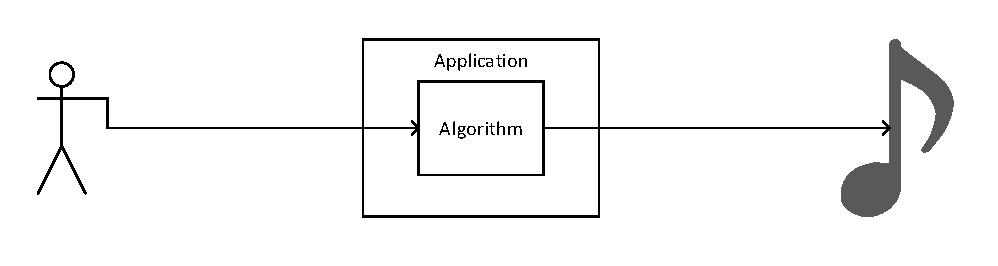
\includegraphics[width=300px]{../images/user-algorithm-audio.pdf}}
\caption{Algorithm as central component}
\label{ims:useralgoaud}
\end{figure}


\begin{figure}
\centerline{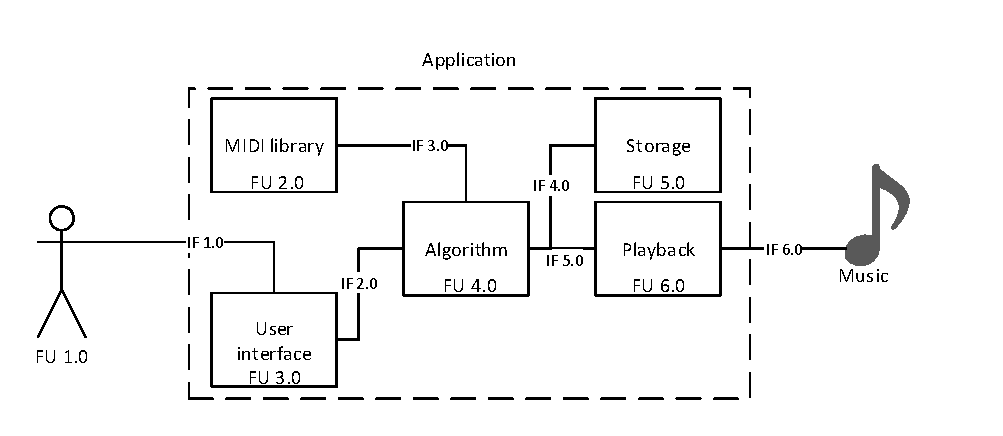
\includegraphics[width=400px]{../images/architecture.pdf}}
\caption{Functional architecture}
\label{ims:funcarch}
\end{figure}

Incorporating all these elements we can concretely describe the project in discrete components in a functional architecture diagram, see figure \ref{ims:funcarch}.

\section{Functional architecture}
\subsection{Functional Unit 1 - Operator}
The operator is responsible for interacting with the application. The operator will select the type of style for composition and instruct to application to compose music.
If a certain piece of music is to be save the operator will be responsible for instructing the application to do so and to select the location the \ac{MIDI} file is to be saved

\subsection{Functional Unit 2 - MIDI library }
The MIDI library is a large collection of \ac{MIDI} files. The files in the \ac{MIDI} library are organized into categories. Each category represents a certain style of music
The algorithm will utilize a subset of the library (a category) as input.

\subsection{Functional Unit 3 - User Interface}
The user interface is the front end of the application. The operator interacts with this functional unit in order to instruct the application what to do.
The user interface should be designed in a user-friendly manner in order to accommodate the operator.
A conceptual user interface is shown in figure \ref{ims:conceptuserinterface}. This user interface allows the user to select a certain style, instruct the algorithm to compose music and to save or play back a piece of music once it is composed.

\subsection{Functional Unit 4 - Algorithm}
The algorithm is the central part of this project. The algorithm converts the input \acp{MIDI} into output \ac{MIDI}.

The algorithm will utilize a category of \ac{MIDI} files from the \ac{MIDI} library in order to compose a new piece of music not in the \ac{MIDI} library.

The output piece of music will represent the style of music that was used as input.
The possible types of algorithms were discussed in section \label{chap:comp_algo}

\subsection{Functional Unit 5 - Storage}
This unit is responsible for storing the output \ac{MIDI} from the algorithm into a \ac{MIDI} file.

\subsection{Functional Unit 6 - Playback}
This unit is responsible for playing back the output \ac{MIDI} from the algorithm through an audio output device

\section{Interfaces}
The interfaces indicate the interaction between different functional units.
The interfaces have the following functions:
\\Interface:
\begin{enumerate}
\item Interface between the user and the user interface. This input would be from a input peripheral device.
\item Interface between the user interface and the algorithm. The interface calls the algorithm with the parameters supplied by the user such as when to start and what type of style was selected
\item Interface between the \ac{MIDI} library and the algorithm. The input to the algorithm is a selection of \acp{MIDI}. The interface converts \ac{MIDI} files into a format required by the algorithm
\item Interface between the algorithm and storage. This interface converts the output from the algorithm into the \ac{MIDI} file format
\item Interface between the algorithm and playback. This interface converts the output from the algorithm into a format that is ready for playback through the playback functional unit.
\item Interface between the playback and the music. This represents the audio output device and it's workings.
\end{enumerate}

\chapter{Operational Flow}

The operational flow indicates the interaction between the operator and the application and how the operator should use it.

\begin{figure}[ht]
\centerline{
\includegraphics[width=400px]{../images/user_interaction.pdf}}
\caption{Interaction with the application}
\label{ims:interactionapp}
\end{figure}

\begin{figure}[ht]
\centerline{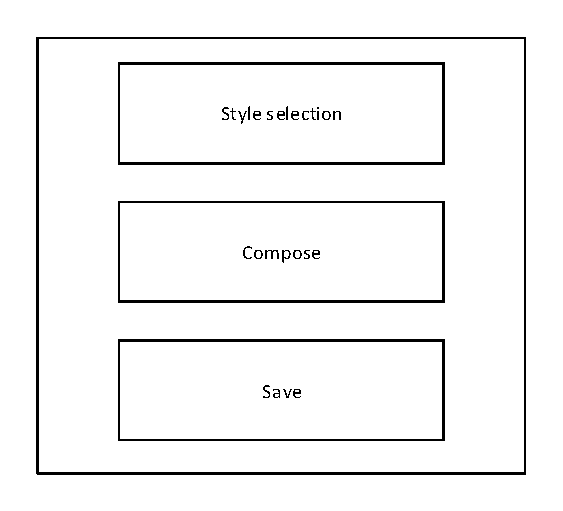
\includegraphics[width=150px]{../images/user_interface.pdf}}
\caption{Conceptual user interface}
\label{ims:conceptuserinterface}
\end{figure}

Figure \ref{ims:interactionapp} shows how the operator interacts with the application. Figure \ref{ims:conceptuserinterface} shows a conceptual user interface with which the operator would interact.

For this application, the operator selects the style of music to be composed. Instructs the application to compose the music according to the selected style and then to instruct the application to either play back the piece of generated music or save it to storage.

\chapter{Algorithms}
In section \label{chap:comp_algo} the following types of music composition algorithms were investigated:
\begin{enumerate}
\item Neural Networks
\item Genetic Algorithms
\end{enumerate}
It was found that the pieces generated by neural networks lack musical coherency and perform poorly as the length of music increases. Some other attempts have met slightly more success although the overarching view for neural networks in music composition seems grim\footnote{Although neural networks as functions in genetic algorithms have had better success}.

The decision was made for genetic algorithms as the main composition algorithm for the following reasons:
\begin{enumerate}
\item They allow for great flexibility in implementation and music representation
\item The majority of research into machine learning music composition has been into genetic algorithm fitness functions
\item Great amount of variety made possible by different fitness functions and by the representation of music used in \acp{GA}
\end{enumerate}

Thus to reiterate, the algorithm employed in the application will be a \ac{GA}. As stated above a large amount of research has been into the fitness functions of different \acp{GA}.

In section \ref{sec:chapfitness} the following fitness functions were covered:
\begin{enumerate}
\item Zipf's law
\item Cosine similarity
\item Neural Networks
\item Normalized Compression Distance
\item Interactive evaluation\footnote{An interactive fitness function imposes a bottleneck on the performance of the system}
\end{enumerate}

\begin{figure}
\centerline{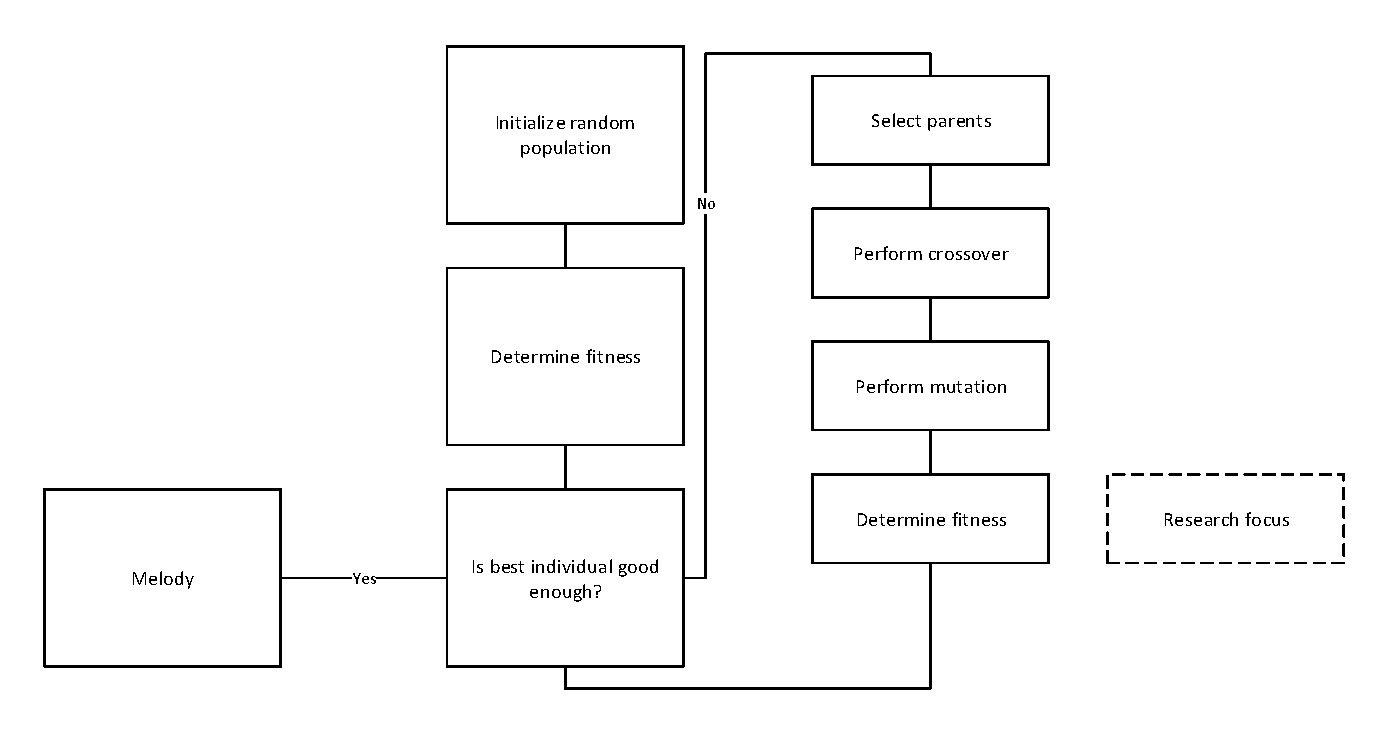
\includegraphics[width=400px]{../images/GA_flow.pdf}}
\caption{Flow diagram of the operation of a genetic algorithm}
\label{ims:geneticflow}
\end{figure}

Figure \ref{ims:geneticflow} indicates the flow for a genetic algorithm/program.

\chapter{Methodology}
For this project a quantitative approach is taken toward algorithmic music composition. In particular quantitative metrics will be used in the fitness function of the genetic algorithm.

\section{Algorithm}
Evolutionary algorithms come in a variety of different types. The two most common types found are Genetic Algorithms and Genetic Programming. Genetic programming has been found to be more suitable than genetic programming due to music forming a hierarchical structure.

A flexible genetic programming model will be developed that is able to function with the investigated fitness functions. 

\section{Fitness functions}
The fitness function is a primary research interest in genetic music composition. An ideal fitness function captures the human perception of pleasantness in music.


Of the set of investigated fitness functions only the following functions will be implemented:
\begin{enumerate}
\item Cosine similarity
\item Neural networks
\item Normalized Compressions Distance
\end{enumerate}
As interactive evaluation is slow and Zipf's law is superseded by Cosine similarity.

\section{Music Representation}
A flexible music representation will also be developed for the genetic programming algorithm. The representation will model \ac{MIDI} events and manipulation of them.
For example:
\begin{lstlisting}
  (d wn :=: f wn :=: a wn) :+:
  (g wn :=: b wn) :+:
  (c bn :=: e bn :=: g bn)
\end{lstlisting}
\begin{figure}
\center
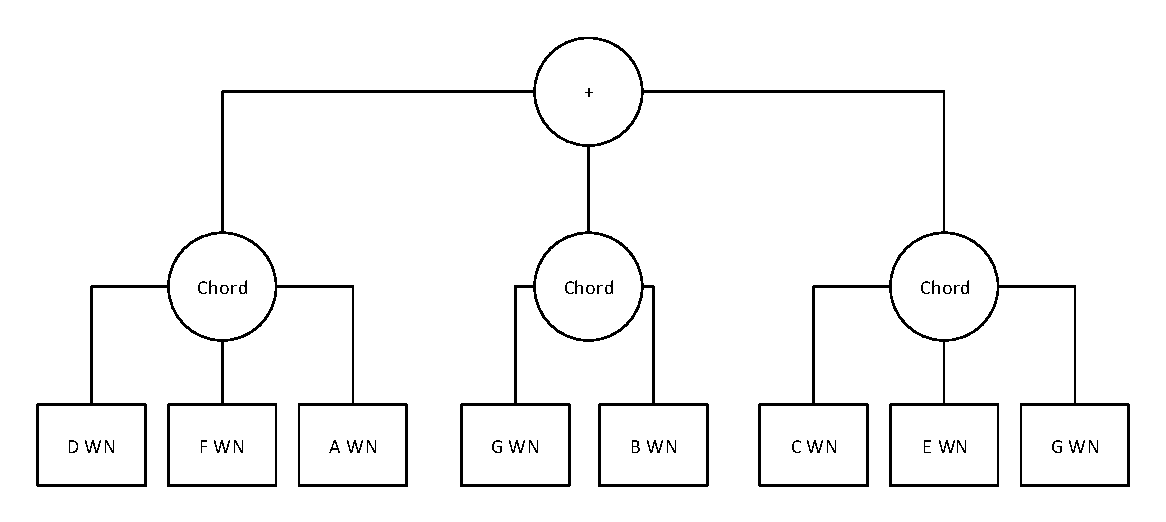
\includegraphics[width=400px]{../images/tree_stuct_piece.pdf}
\caption{A music piece in a tree structure}
\label{ims:musicpieceextrree}
\end{figure}
Where the :=: operator indicates pieces are played in parallel (chords) and :+: indicates pieces are played in series. a,b,d,e,f,g indicate the note pitch and wn indicates a whole note.
Figure \ref{ims:musicpieceextrree} indicates this in tree form. Strictly a chord is a set of three or more notes that are played simultaneously. Note that the second branch is only constituted of two notes.

Minsky and Laske \cite{Minsky1992} argued for a tree representation of music since the tree represents the hierarchical nature of music. The tree representation is much more complex than data structures such as vectors that are used in \acp{GA}.

Some authors \cite{Biles1994} limit the search space by ensuring that melodies are in a certain scale 

\section{Genetic operators}
Several different operators can be performed on the tree structure. In figure \ref{ims:musicpieceextrree} the serial concatenation and parallel concatenation operators were shown.
Some additional operators which may be employed include:
\begin{itemize}
\item Repetition - Repeating a segment a given number of times
\item Shift note pitches - Shift all pitches of notes by a certain amount
\item Duration elongation or contraction - For example a slow operation doubles the duration
\item Transposition - Moving note positions relatively
\item Retrograde - Reversed order of notes
\end{itemize}

Genetic operations such as mutation and crossover may be used conventionally.

\chapter{Metrics} \label{chap:metrics}
Feature extraction is required to reduce the search space and to provide the fitness function with musically meaningful measures with which to rate the fitness. In this section we cover some quantitative metrics that may be used as measures to identify or represent music.

The different types of metrics that will be used include:
\begin{enumerate}
\item Pitch - List of pitches
\item Pitch differences - Store first pitch, thereafter list consecutive pitch differences
\item Chromatic tone - 12 pitch class. Notes are reorganized into 12 classes.
\item Note durations - durations of notes
\item Pitch distance - intervals between repetition of pitches
\item Chromatic tone distance - intervals between repetition of chromatic tones  
\item Melodic interval - intervals between the current note and the previous note
\item Melodic bi-gram - Pairs of melodic intervals
\item Rhythm - duration of a note in addition to the following rest
\item Rhythmic interval - relationship between adjacent note rhythms
\item Rhythmic bi-gram - Pairs of adjacent rhythmic intervals.
\end{enumerate}

Let $p$ denote the pitch of the note, where $0 \leq p < 128$.
Then the chromatic tone is given by:
\[c = p \% 12\]
where $\%$ indicates the modulo operation.
The melodic interval is given by:
\[\text{mi}_k = p_k - p_{k-1} \]
The melodic bi-gram is given by:
\[b_k = (\text{mi}_k, \text{mi}_{k+1}) \]
Let $r$ indicate the note duration with rests
Then the rhythmic interval is given by:
\[\text{ri}_k = \frac{r_k}{r_{k-1}} \]
and the rhythmic bigram
\[\text{rk}_k = (\text{ri}_k, \text{ri}_r) \]

In this manner we can build a metric vector, let $m_i(A)$ denote a metric's value at position $i$ for musical piece $A$. Then the metric vector is given by $\vec{M}_A = \{m_0(A), m_1(A), \ldots, m_n(A) \}$ 



\chapter{Fitness functions}
\section{Cosine similarity}
Some fitness functions such as Cosine similarity and Zipf's law operate on the features of music. 

Cosine similarity can be applied to the metrics listed in section \ref{chap:metrics}. Let $\vec{M_A}$ denote the vector of metric values according to a metric $m$ for a music piece $A$ and $\vec{M_B}$ denote the vector by $m$ for a music piece $B$ then the similarity between $A$ and $B$ is given by:
\[\text{similarity}_m(A,B) = \frac{\vec{a} \cdot \vec{b}}{|\vec{a}| |\vec{b}|}\]

A set of metrics may be used. 
The fitness function is then given by:
\[f = \sum_{k} w_k \times \text{similarity}_{mk}(A,B) \]
where $w$ is a weight assigned to metric $mk$.

\section{Normalized compression distance}
In order to utilize \ac{NCD} both pieces being tested need to be encoded in the same way. Musical pieces may be encoded as metric vectors as listed in section \ref{chap:metrics}.

\ac{NCD} was covered in section \ref{sec:class_ncd}.

In order to utilize the \ac{NCD} as a fitness function the following steps are taken:
\begin{enumerate}
\item Encode a set from the \ac{MIDI} library according to a metric. Let $\Omega = \{\vec{M_0}, \vec{M_1}, \ldots, \vec{M_n}\}$ for musical pieces $0$ to $n$ in the \ac{MIDI} library that accord to a certain style.
\item Encode the population individual $x$ according to the metric (Given by $\vec{M_x}$).
\item Employ the fitness function
\end{enumerate}

The fitness function that will be used is:
\[f(x) =  \left(\sum_{\vec{T}\in\Omega} \text{NCD}(\vec{M_x}, \vec{T}) \right)\]

\chapter{Conclusion}
In order to solve the problem of generating music algorithmically the task was broken down into its functional architecture. From this each functional unit and its interaction is made apparent. The core component of this project is the algorithm which is used to compose music

The decision was made to utilize a genetic programming algorithm since the tree structure accommodates the hierarchical nature of music. Genetic programming provides flexibility, variety of possible styles and a large amount of research has been done one fitness functions for genetic algorithms.

Fitness functions require good measures that make it possible to rate musical pieces quantitatively. A set of metrics were developed in which musical pieces can be measured.

Two fitness functions, namely Cosine similarity and \ac{NCD} were developed to incorporate these metrics.